\section{Physical question and scope}
In the Berger--Hopf interpretation, gravitational lensing is the optical
response of an envelope event traversed by environmental radiation. The
calculation relates prepared incoming light to its outgoing observables,
conditional on the envelope state and surrounding geometry. Light is the
probe of that state dependence. Traversal alone supplies no claim of
encapsulation, de-encapsulation, reflection, absorption or a new photon law.

The quantitative question is whether a change in the encounter geometry or
envelope state produces image positions and relative arrival times that
survive the available source, galaxy and environmental degeneracies.
We retain two explicit realizations: a conventional galaxy-potential
benchmark, and a response constructed from the existing Berger--Hopf metric
and optical equations. The first executable comparison holds the galaxy
encounter fixed and applies the available smooth geometric correction.
An action-derived replacement for the local galaxy encounter remains a
separate unresolved calculation. A restricted zero response and an exact
degeneracy are valid outcomes of the declared comparison.

This focused draft develops the accepted contribution to ``Strong
Gravitational Lens Modeling,'' with submission intended by 25 February 2027.
It uses the inherited frozen R1 background within its supported domain
$0\leq z\leq2.1$. It does not admit the current muon preparation as a lensing
calibration. No equation evaluated below requires restarting that
preparation or an inclusive pair-production four-point calculation.

\section{Matched optical experiment}
\label{sec:sl-experiment}
The observer, lens and source carry orthonormal local tetrads. Two Sachs
screen vectors are parallel transported along a common fiducial ray;
transverse coordinates are physical lengths in those screens and angles
are radians in the local observer or lens frame. We normalize the
past-directed affine ray by the observer frequency magnitude
$\omega_o=|u_o\!\cdot k_o|=1$ and use positive
$1+z_a=\omega_a/\omega_o$. The photon wavelength is assumed much smaller
than the metric and encounter scales. Null propagation, not an additional
photon interaction law, determines the transfer.

The source emits the same narrow transient marker with the same emission
phase, local spectrum, polarization and transverse source coordinate $s$ in both
realizations. Its small-amplitude stress is neglected as a test beam.
The reference observed central wavelength is $550\,{\rm nm}$; at the fixed
source redshift the corresponding emission wavelength is $275\,{\rm nm}$.
The entrance and exit surfaces of the local encounter are planes in the
lens rest frame, normal to the fiducial ray, outside the region assigned
to the thin galaxy potential. Their thin-plane limit is the lens screen.
Propagation outside this encounter uses the smooth reference geometry.
The observable is the direction of each received image and the observer
proper-time separation between copies of the same marker. Absolute
unlensed travel time and a common source-dependent arrival constant are
not measured.

The matching prescription fixes the transverse physical source coordinate,
the galaxy's physical parameters and the measured lens/source redshifts
$z_l=0.3$ and $z_s=1.0$. The reference redshift-selected screens consequently
move when the metric response changes. At each perturbation images are
solved again. Since
\begin{equation}
 s=D_{os}\beta,\qquad x=D_{ol}\theta,
 \label{eq:sl-source}
\end{equation}
holding $s$ fixed gives
\begin{equation}
 \delta\beta=-D_{os}^{-1}\delta D_{os}\,\beta.
 \label{eq:sl-deltabeta}
\end{equation}
Fixing $s$, $\beta$ and the image positions independently would describe
inconsistent experiments. An alternative fixed inferred angular source
is a different protocol and must be labeled accordingly.
The longitudinal position and emission event follow each realization's
fixed observed-redshift source surface. The physical matching holds the
transverse displacement fixed; it does not additionally fix a complete
three-dimensional source world-line across the varied geometries.

Cosmological radiation-fluid perturbations $(\delta_r,v_r)$ belong to the
background state, not to this incoming optical pulse. Muon/reference-state
covariances are a third object. Fixing the pulse does not fix its outgoing
field or an induced interface response.

\section{Coupled state and metric response}
\label{sec:sl-coupled}
The frozen background parameters are
\begin{equation}
 (\Omega_{m0},\Omega_{r0},\Omega_{k0})=(0.31,9\times10^{-5},-0.018),
 \quad H_0=67.4\ {\rm km\,s^{-1}Mpc^{-1}},
\end{equation}
with retained action parameters $\lambda=1$, $q=3$ and
$V_0/(\Mpl^2H_0^2)=2.3986073449708067$. The background is reused without
new shooting, calibration or broad stability scans.

For a selected normalized $n=2$ real spatial harmonic, the physical anchor
at $z_i=2.1$ is
\begin{equation}
 Y_i=(\zeta_i,\Pi_{2i},\delta^{\rm ADM}_{mi},
 \delta^{\rm ADM}_{ri},v^{\rm ADM}_{mi},v^{\rm ADM}_{ri})^T.
 \label{eq:sl-anchor}
\end{equation}
The nine-dimensional spatial $n=2$ eigenspace is not reduced to two
physical amplitudes. Selecting one spatial profile leaves six initial
amplitudes. The historical two-column seed sets the four ADM fluid
coordinates to zero and selects a restricted slice.

For the observer-dipole profile on a reference sphere of radius $R_H$,
one possible normalized choice is
\begin{equation}
 Q_{\hat p}(\psi,\hat n)=\frac{\sqrt3}{\pi R_H^{3/2}}
 \sin(2\psi)\,\hat n\!\cdot\!\hat p,
 \quad \int_{S^3(R_H)} Q_{\hat p}^2\dd V=1.
 \label{eq:sl-profile}
\end{equation}
The dimensionless unit-sphere convention removes $R_H^{-3/2}$.
The selected sky axis $\hat p$ is a conditional input, not a direction
selected by an isotropic background or by the previous supernova fits.
Its radius convention must agree with that of the action provider.

The action-native ADM plus Schutz--Sorkin implementation uses
$x=(\zeta,D_m,D_r)$, with
$D_m=\delta_m^{\rm ADM}+3\zeta$ and
$D_r=3\delta_r^{\rm ADM}/4+3\zeta$.
For auxiliary variables $u=(\alpha,\chi,v_m,v_r)$,
\begin{equation}
 \frac{L_2}{a^3}=\frac12u^TAu+u^T(B\dot x+Dx)
 +\frac12\dot x^TK_0\dot x+\frac12x^TEx.
 \label{eq:sl-action}
\end{equation}
Constraint elimination gives
\begin{align}
 u&=-A^{-1}(B\dot x+Dx),&
 M&=K_0-B^TA^{-1}B,\nonumber\\
 L&=-B^TA^{-1}D,&V&=E-D^TA^{-1}D,\nonumber\\
 p&=a^3(M\dot x+Lx),&
 \dot x&=M^{-1}(a^{-3}p-Lx),\label{eq:sl-canonical}\\
 \dot p&=a^3(L^T\dot x+Vx).\nonumber
\end{align}
These are the coupled original action applications evolved by the provider.
The anchor definition
$\Pi_2=2a_i^3G_{S,2}(t_i)\dot\zeta_i$ is reference-normalized;
it is generally not $p_\zeta$. The ADM fluid continuity constraints set
$\dot D_I=k_n^2(v_I-\chi)$ with the provider's closed-harmonic factor.
Thus the reference normalization, reconstructed auxiliaries and
Eq.~\eqref{eq:sl-canonical} define the anchor-to-canonical map together.
No independent momentum identification is imposed.

The reconstructed Newtonian rows use
\begin{equation}
 \dd s^2=-(1+2\Phi)\dd t^2
 +a^2(1-2\Psi)\gamma_{ij}\dd x^i\dd x^j,
 \qquad \Phi_W=\frac{\Phi+\Psi}{2}.
 \label{eq:sl-metric}
\end{equation}
Potential rows, harmonic normalization and time units are checked before
composition. Legacy growth and luminosity-distance modules require a sign
and provider adapter; their arrays are not substitutes for the coupled
response at this state.

\section{Three propagation maps and relative arrival times}
\label{sec:sl-propagation}
For a null tangent and parallel screen, the Jacobi application is
\begin{equation}
 \frac{\dd^2J_a}{\dd\lambda^2}=\mathcal T(\lambda)J_a,
 \quad (J_a,J_a')|_{\lambda_a}=(0,\omega_a I),
 \quad \mathcal T_{AB}=-R_{\mu\nu\rho\sigma}
 e_A^\mu k^\nu k^\rho e_B^\sigma.
 \label{eq:sl-jacobi}
\end{equation}
Then $D_{ab}=J_a(\lambda_b)$ maps angles in the frame at $a$ to physical
separations at $b$. The three maps $D_{ol}$, $D_{os}$ and $D_{ls}$ use one
reference geometry and compatible frequency/screen normalization.
Here $J_a$ already includes the initial factor $\omega_a$; it is not
multiplied by that factor a second time. For reverse transport with the
same oriented affine derivative, reciprocity reads
$D_{ba}/\omega_b=-(D_{ab}/\omega_a)^T$. If the reverse angular opening is
instead initialized toward the past endpoint, its derivative has the
opposite sign and the positive physical reverse map obeys the corresponding
plus-sign relation. The implemented reverse check uses that positive map.
In closed FLRW they reduce to
\begin{equation}
 \overline D_{ab}=a_b S_K(\chi_b-\chi_a)I,
 \qquad S_K(r)=\frac{\sin(\sqrt K r)}{\sqrt K}.
 \label{eq:sl-flrw-distance}
\end{equation}
In particular $D_{ls}$ is independently initialized at the lens, not the
difference $D_{os}-D_{ol}$. The main encounter is omitted from all three
reference maps when represented as a separate potential.

The existing seven-state reduction is recovered by writing the conformal
Jacobi map as $S_K(I+\mathcal A)$, with
$\mathcal A=-\kappa I-\left(\begin{smallmatrix}
\gamma_1&\gamma_2\\\gamma_2&-\gamma_1\end{smallmatrix}\right)$.
The directly evaluated sources give
\begin{equation}
 Z'=\mathcal Z,\qquad
 \kappa''+2\frac{C_K}{S_K}\kappa'=\mathcal F,\qquad
 \gamma_A''+2\frac{C_K}{S_K}\gamma_A'=\mathcal G_A,
 \label{eq:sl-seven}
\end{equation}
where $C_K=S_K'$, $\mathcal F=-\tr\delta\mathcal T/2$,
$\mathcal G_1=-(\delta\mathcal T_{11}-\delta\mathcal T_{22})/2$ and
$\mathcal G_2=-\delta\mathcal T_{12}$ in the rescaled conformal system.
These fixed-coordinate path variables are passed through
Eq.~\eqref{eq:sl-endpoint} before asserting a fixed measured-redshift
response. They are not themselves a complete observed-redshift arrival
kernel.

For the declared axial profile, the executed transport differentiates the
original angular geodesic equation as an independent construction of the
screen maps. Put $q(\chi)=Q_{\hat p}(\chi/R_H,\hat p)$,
$P_g=1+2\Phi q$, $M_g=1-2\Psi q$, $A=a\sqrt{P_g}$ and
$B_g=a\sqrt{M_g}$. In conformal coordinates
$\dd s^2=-A^2\dd\eta^2+B_g^2(\dd\chi^2+S_K^2\dd\Omega^2)$.
With $N=\ln a$ and static-tetrad frequency $E$, the equations evaluated are
\begin{align}
 N_{,\chi}&=-aH\sqrt{M_g/P_g},\nonumber\\
 (\ln E)_{,\chi}&=aH\sqrt{M_g/P_g}
 -\frac{aH\Psi_{,N}q}{\sqrt{M_gP_g}}
 -\frac{\Phi q_{,\chi}}{P_g},
 &\lambda_{,\chi}&=B_g/E,\label{eq:sl-axial-ray}\\
 \vartheta_{,\chi}&=\frac{L_\vartheta}{B_gS_K^2E},
 & (L_\vartheta)_{,\chi}&=EB_g a^2q
 \left(\frac{\Phi}{A^2}+\frac{\Psi}{B_g^2}\right)\vartheta,
 \qquad D=B_gS_K\vartheta.\nonumber
\end{align}
The matter tetrad follows the action-native velocity-potential convention
$u_\chi=v_m q_{,\chi}$, rather than an unadapted legacy velocity row.
For $s_u=u_\chi/B_g$ and $\gamma_u=\sqrt{1+s_u^2}$,
$\omega=E(\gamma_u+s_u)$. Observed-redshift endpoints are roots of
$\omega=1+z$. Observer initialization includes the corresponding aberration
$\vartheta_o=\gamma_{uo}+s_{uo}$; at the moving lens,
$\vartheta_l=0$ and $L_{\vartheta l}=B_{gl}S_{Kl}\omega_l$.
Both screen maps coincide on this axis by rotation symmetry.
In particular the angular forcing term in
Eq.~\eqref{eq:sl-axial-ray} is retained: suppressing it because the selected
profile is a dipole would miss its focusing and endpoint response.
Finite perturbations use this explicitly declared truncated metric only
to check first derivatives; they are not nonlinear cosmological solutions.

A separate conformal Jacobi control applies the inherited seven-state
equation to all six anchor columns, with axial shear zero and forcing
\begin{equation}
 \mathcal F=q(\Psi''-8K\Psi)
 +2\Psi'(q'+H_Kq)+(\Psi-\Phi)\frac{q}{S_K^2},
 \qquad H_K=C_K/S_K.
 \label{eq:sl-seven-control}
\end{equation}
Primes here differentiate along the background $\chi$ ray. This is the
stable harmonic form of
$(\Psi q)''+2H_K(\Psi q)'-q(\Phi+\Psi)/S_K^2$; it retains the angular
geodesic term. Its observer initialization includes the matter-tetrad
aberration. The measured-redshift endpoint response is then
$\delta\ln D_{ob}=\delta N_b+H_{Kb}\delta\chi_b-\kappa_b$, which is
compared with the independently varied physical maps for $b=l,s$.
The $\zeta_\gamma$ slot is unused and zero in this conformal control;
the complete physical frequency and endpoint motion come from the metric
ray of Eq.~\eqref{eq:sl-axial-ray}. A zero control slot therefore carries
no assertion of a zero redshift response.

With $\hat\alpha=\nabla_x\hat\psi$ in the lens frame, the matrix lens and
arrival-time equations are
\begin{align}
 \beta&=\theta-D_{os}^{-1}D_{ls}\hat\alpha(D_{ol}\theta),
 \label{eq:sl-lens}\\
 T&=(1+z_l)D_{ol}^TD_{ls}^{-1}D_{os},
 \label{eq:sl-T}\\
 ct(\theta,\beta)&=\frac12(\theta-\beta)^TT(\theta-\beta)
 -(1+z_l)\hat\psi(D_{ol}\theta)+f(\beta).
 \label{eq:sl-arrival}
\end{align}
This is the physical angle-to-separation normalization of the arbitrary
reference-spacetime formalism of
\citet[Eqs.~(2), (3), (11)--(14)]{Fleury2021arbitrary}.
Their frequency-weighted affine maps become the $D_{ab}$ used here.
Reciprocity implies symmetry of $T$ when all maps come from the same
reciprocal transport. The numerical antisymmetry residual is inspected
before any arrival calculation. Arbitrary symmetrization would conceal an
incompatible propagation input. Only differences $t_A-t_B$ are used, so
$f(\beta)$ cancels.

\subsection{Measured redshifts and moving initialization}
The accumulated photon redshift response is
$Z_a=\delta\ln(1+z_a)|_{\lambda_a}$. Holding the measured redshift fixed
moves the coordinate endpoint by
\begin{equation}
 \delta\lambda_a=-\frac{Z_a}{(\ln\overline\omega)'_a},
 \qquad
 \delta\chi_a=-\frac{Z_a}{\mathcal H_a}
 \quad\hbox{in background conformal distance}.
 \label{eq:sl-endpoint}
\end{equation}
Observer tetrad, source/lens velocity and gravitational frequency terms
belong in $Z_a$ for the chosen state. The map variation obeys
\begin{equation}
 (\delta J_a)''=\mathcal T_0\delta J_a+\delta\mathcal T\,J_{a0},
 \quad
 \delta J_a|_a=-\omega_a I\delta\lambda_a,
 \quad (\delta J_a)'|_a=\delta\omega_a I.
 \label{eq:sl-moving-init}
\end{equation}
At its output one also adds $J_{a0}'(\lambda_b)\delta\lambda_b$ and the
required screen/frame conversion. The zero of $J_{a0}$ at its initial
point removes the apparent $J_{a0}''\delta\lambda_a$ term there.
Equation~\eqref{eq:sl-moving-init} is essential for $D_{ls}$; retaining
only a fixed-affine Green integral does not give the measured-redshift
observable. A frequency normalization expressed in physical angles must
move with the initialization as well.

\subsection{Complete first variation}
Write $q=\theta-\beta$ and permit a physical encounter change
$\delta\hat\psi|_x$. At a stationary image, varying
Eq.~\eqref{eq:sl-arrival} gives
\begin{align}
 c\delta t={}&\frac12q^T\delta Tq-q^TT\delta\beta
 -\delta z_l\hat\psi(x)\nonumber\\
 &-(1+z_l)\left[
 \hat\alpha(x)^T\delta D_{ol}\theta+\delta\hat\psi|_x\right]
 +\delta f(\beta),
 \label{eq:sl-complete-variation}\\
 \delta T={}&\frac{\delta z_l}{1+z_l}T
 +(1+z_l)\big[\delta D_{ol}^TD_{ls}^{-1}D_{os}
 +D_{ol}^TD_{ls}^{-1}\delta D_{os}\nonumber\\
 &\hspace{28mm}-D_{ol}^TD_{ls}^{-1}
 \delta D_{ls}D_{ls}^{-1}D_{os}\big].\nonumber
\end{align}
The image-position derivative cancels by stationarity;
the source-coordinate and physical lens-impact terms do not.
For the matched fixed-redshift protocol $\delta z_l=0$, while endpoint
shifts remain inside the map changes. If a local envelope potential has
not been derived, its $\delta\hat\psi|_x$ is unresolved, rather than
implicitly supplied by a smooth cosmological response. The executed
correction holds the physical conventional encounter fixed and sets this
term to zero by the definition of that restricted comparison.

\section{Conventional encounter and analytic control}
\label{sec:sl-galaxy}
The numerical realization uses a singular isothermal sphere (SIS), with
one-dimensional velocity dispersion $\sigma_v=220\,{\rm km\,s^{-1}}$:
\begin{equation}
 \hat\psi(x)=b_{\rm phys}|x|,
 \quad b_{\rm phys}=4\pi\frac{\sigma_v^2}{c^2},
 \quad \theta_E=b_{\rm phys}\frac{D_{ls}}{D_{os}}.
 \label{eq:sl-sis}
\end{equation}
Here $\hat\psi$ has dimensions of length and $b_{\rm phys}$ is a
dimensionless deflection amplitude. For scalar distances and
$0<\beta<\theta_E$, the two images and positive saddle-minus-minimum delay
are
\begin{equation}
 \theta_\pm=\beta\pm\theta_E,
 \qquad \Delta t_{-+}=\frac{2D_{\Delta t}}{c}\theta_E\beta,
 \quad D_{\Delta t}=(1+z_l)\frac{D_{ol}D_{os}}{D_{ls}}.
 \label{eq:sl-sis-control}
\end{equation}
The source is away from the caustic and the central singularity.
Its baseline position is $\beta_0=(0.2\theta_{E0},0)$ and its held-fixed
physical screen coordinate is $s=D_{os,0}\beta_0$. A smooth encounter
control uses the same strength in
$\hat\psi(x)=b_{\rm phys}\sqrt{|x|^2+r_c^2}$ with
$r_c=0.05\,{\rm kpc}=5\times10^{-5}\,{\rm Mpc}$. Its central image,
when present, is retained in the image census rather than discarded to
imitate the singular two-image case.
The SIS is an illustrative conventional galaxy model, not an inferred mass
distribution or a fit to observations. A local encounter specified by
Eq.~\eqref{eq:sl-sis} is counted once, outside the reference Jacobi maps.

\section{Envelope construction and the available channel}
\label{sec:sl-envelope}
The inherited constitutive chain is
\begin{align}
 \mathcal L_\psi\psi&=J_{\rm grav}+\mathcal E_\Sigma[Q_\Sigma]+\xi,
 & h_{\rm topo}&=\mathcal R_{g\psi}\psi,\label{eq:sl-envelope-chain}\\
 \mathcal R_{g\psi}&=-\mathcal A_g^{-1}\mathcal B_{g\psi},
 &Q_\Sigma&=\frac{c^2}{8\pi}\int_{\Sigma_\star}
 H_\Sigma\Delta K_{uu}\dd A.\nonumber
\end{align}
The inverse and projections require the same physical constraint domain,
boundary conditions and state. In the retained static spatial limit,
$\mathcal L_\psi$ reproduces $-\nabla^2+B\nabla^4$. The static seam export
has the inherited radial shape
\begin{equation}
 \mathcal E_\Sigma^{(0)}[Q_\Sigma]
 =\epsilon_\Sigma\frac{Q_\Sigma}{Q}
 \frac{\Theta(r-r_\star)}{r^2}.
 \label{eq:sl-static-seam}
\end{equation}
Its common-action normalization and orientation remain unresolved.
The time derivative of this source for a moving seam is a proposed
kinematic continuation; it is not used as an action-selected optical
interaction in this checkpoint.

For normalized physical metric basis columns $P_g=(e_A,e_\psi)$ and a
normalized local topographic profile $\varphi$, define
\begin{equation}
 A_g^{\rm loc}=P_g^\dagger\widehat H_{gg}P_g=
 \begin{pmatrix}a&b\\b&c\end{pmatrix},
 \quad B_{g\psi}^{\rm loc}=P_g^\dagger\widehat H_{g\varphi}\varphi
 =\binom uv.
 \label{eq:sl-local-hessian}
\end{equation}
The inverse application and local Schur curvature are
\begin{align}
 \mathcal R_{g\psi}^{\rm loc}
 &=\frac{1}{ac-b^2}\binom{bv-cu}{bu-av},
 &\Delta_g&=ac-b^2\ne0,\label{eq:sl-local-response}\\
 k_{\rm loc}&=c_\varphi-(B_{g\psi}^{\rm loc})^T
 (A_g^{\rm loc})^{-1}B_{g\psi}^{\rm loc},
 &c_\varphi&=\langle\varphi,\widehat H_{\varphi\varphi}\varphi\rangle.
 \nonumber
\end{align}
The diagnostic is
$\|A_g^{\rm loc}\mathcal R_{g\psi}^{\rm loc}+B_{g\psi}^{\rm loc}\|$,
with the determinant, basis norms, Legendre gate and boundary-domain status
reported. These coefficients are action projections, not free fitting
parameters. The cosmological lapse/shift auxiliary Hessian in
Eq.~\eqref{eq:sl-action} does not automatically supply this local physical
metric/topographic Hessian.

The available same-domain action projection is nevertheless executed on
the ADM auxiliary block at $z_l=0.3$. After eliminating the fluid velocity
auxiliaries its lapse/shift entries, in the action-density convention
$L_2/a^3$ and unit normalized harmonic coordinates, are
\begin{equation}
 (a_{\rm ADM},b_{\rm ADM},c_{\rm ADM})
 =(-7.96725028,\ 0.56954480,\ 0.48267978),
 \qquad \det A_{\rm ADM}=-4.17001193.
\end{equation}
All six mixed source columns are evaluated; their inverse response has
residual $1.42\times10^{-15}$, the original action constraints have maximum
residual $5.28\times10^{-16}$ and the Schur reduction agrees with the native
reduced action to $4.16\times10^{-16}$. The unit $\zeta$ source has
pre-elimination self entry $0.301115412$ and Schur entry $5.097094780$.
The reduced kinetic eigenvalues are $(0.00418211,0.17251064,0.43386354)$,
so its Legendre gate is satisfied at this event. These data preserve the
common cosmological domain and demonstrate its actual auxiliary inverse
application. The map
$\Phi=\alpha+\dot\chi$, $\Psi=-\zeta-H\chi$ depends on state and time
derivatives, so it cannot rename this block as the local physical
$A_g^{\rm loc}$ of Eq.~\eqref{eq:sl-local-hessian}.

In the established static block-diagonal spatial phase channel the mixed
source is explicitly
\begin{align}
 \mathcal S_{ij}[j,\varphi]={}&
 2F''(X)(j^k\nabla_k\varphi)A_{ij}
 +2F'(X)j_{(i}\nabla_{j)}\varphi
 -F'(X)g_{ij}(j^k\nabla_k\varphi),\nonumber\\
 (u,v)&=\int\dd\mu_g\,w\,
 \big((e_A)^{ij},(e_\psi)^{ij}\big)\mathcal S_{ij}.
 \label{eq:sl-static-current}
\end{align}
For $j_i=0$, or for $\nabla_i\varphi=0$, the pointwise source and both
projections vanish exactly. On any invertible admissible metric block this
gives $\mathcal R_{g\psi}^{\rm loc}=0$ and
$k_{\rm loc}=c_\varphi$. This is a channel-specific null result; it does
not determine a nonzero-current state or prove that all lensing vanishes.
No new channel is introduced to manufacture a signal.
For a constant texture admitted by the domain, the phase-invariant
$F(X)$ sector also has zero self entry; other action and boundary terms
must be included before identifying the complete $c_\varphi$.

The smooth coupled cosmological metric response is separately available
from Eqs.~\eqref{eq:sl-action}--\eqref{eq:sl-metric}. Its transfer per anchor
amplitude is a conditional state sensitivity. Until a physical envelope
state and the common-domain local coefficients are supplied, that
sensitivity is neither a galaxy-replacement amplitude nor a calibrated
BHSM prediction.

\section{Nuisance projection and distinguishability}
\label{sec:sl-identifiability}
Let the local observable vector contain the image coordinates and independent
relative delays. In the linearized model
\begin{equation}
 y=BX+N\eta+\epsilon,\qquad
 WCW^T=I,\quad P=I-(WN)(WN)^+,
 \quad F=(WB)^TP(WB),
 \label{eq:sl-fisher}
\end{equation}
$B$ contains conditional physical-state columns, while $N$ contains source
coordinates, galaxy parameters, mass-sheet scale, independent line-of-sight
contributions and cosmological nuisance columns admitted by the declared
protocol. The covariance $C$ is a specified illustrative measurement
covariance, not an estimated observational likelihood. Singular values of
$PWB$ report the surviving rank and parameter-space null directions.
On a null direction there is no likelihood-derived finite uncertainty.
The zero eigenvalue of a Fisher pseudoinverse must not be reported as a
zero error bar. A prior must be added and identified before it can supply
missing information.

For a reduced scalar lens the mass-sheet transformation is
\begin{equation}
 \psi_\lambda(\theta)=\lambda\psi(\theta)
 +\frac{1-\lambda}{2}|\theta|^2,
 \quad \beta_\lambda=\lambda\beta,
 \quad \Delta\phi_\lambda=\lambda\Delta\phi.
 \label{eq:sl-mst}
\end{equation}
It preserves image positions under the corresponding source rescaling.
An independent unrestricted delay scale for each lens absorbs a common
rescaling of all its delays. More sky directions alone do not remove
that freedom. Delay ratios can remove a common scale only where multiple
independent delays exist; a two-image SIS has just one independent delay.
Image distortions or independent environmental/kinematic data require
their own response and likelihood.

The dominant-lens treatment permits subcritical line-of-sight corrections
beyond a single external convergence/shear
\citep{Fleury2021los}. In particular observer--lens, observer--source and
lens--source segments enter differently; treating only the observer--source
convergence can bias cosmographic inference
\citep{Teodori2022}. Their physical contributions are already contained in
the three reference maps here and are not added again as a second
convergence potential. An independent nuisance column represents uncertainty
in an included contribution, not another copy of its mean.

The familiar $H_0^{-1}$ delay scaling follows when dimensionless expansion
history, reduced angular galaxy parameters and angular source coordinates
are fixed: every distance scales as $H_0^{-1}$. Holding the physical source
coordinate fixed instead changes $\beta$, and therefore requires the full
variation in Eq.~\eqref{eq:sl-complete-variation}. The two conventions are
not interchangeable.
In the scale-free SIS control, the fixed physical transverse source gives
an exact first-order cancellation of the delay response to $\ln H_0$.
The independently checked fixed angular-source convention instead gives
$\partial\Delta t/\partial\ln H_0=-\Delta t$.

A pure sky dipole has zero trace-free angular Hessian at Born order,
$(\nabla_a\nabla_bQ)^{\rm TF}=0$; its shear null does not remove its
redshift or isotropic focusing response. Likewise, for $m$ coherent global
amplitudes and a fixed response $M_O$,
\begin{equation}
 C_O^{\rm topo}=M_OC_qM_O^T,\qquad
 \rank C_O^{\rm topo}\leq\rank C_q\leq m.
\end{equation}
This bound concerns the isolated coherent contribution. One local random
field with independent increments can generate many nonparallel response
columns and need not have rank one. No Gaussian factorization of a dressed
state or substitution of a retarded kernel for a statistical state kernel
is used.

\section{Executed numerical checkpoint}
\label{sec:sl-results}
The generated table below is tied to the input manifest and machine-readable
calculation rather than to a manuscript-only amplitude choice. Conditional
perturbations use the same source convention as the benchmark. Centered
finite changes re-solve the image equation independently before comparing
arrival-time differences with Eq.~\eqref{eq:sl-complete-variation}.
\IfFileExists{tables/strong_lensing_results.tex}{%
 \begin{center}\begin{tabular}{p{0.47\linewidth}p{0.46\linewidth}}
\toprule
Quantity & Executed result \\
\midrule
Lens/source redshift & $0.3 / 1.0$ \\
$D_{ol},D_{os},D_{ls}$ [Mpc] & 945.162839, 1689.312240, 1076.994348 \\
SIS image $x$ positions [arcsec] & 1.0678831, -0.7119220 \\
SIS relative delay [days] & 17.09453205 \\
Free-nuisance surviving state rank & 0 \\
Fixed-nuisance control rank & 3 \\
Synthetic-prior-assisted rank & 3 \\
Static spatial phase $(u,v)$ & $ (0,0)$ under the stated current gate \\
\bottomrule
\end{tabular}
\end{center}%
}{\noindent\textit{Results table has not yet been generated. No numerical
prediction is inferred from this placeholder.}}

The physical background maps are
\begin{equation}
 (D_{ol},D_{os},D_{ls})
 =(945.162839,1689.312240,1076.994348)\,{\rm Mpc}.
\end{equation}
The source-screen displacement is $(1.457663367,0)\,{\rm kpc}$.
The SIS images are $(1.0678830532,0)$ and $(-0.7119220355,0)$ arcsec, with
relative delay $17.0945320516$ days. Their original lens-equation residual
is below $8.5\times10^{-22}$ radians and their arrival stationarity residual
is zero at reported floating precision. The analytic scalar SIS delay
agrees within $1.1\times10^{-14}$ days. Baseline segment reciprocity
residuals are below $9\times10^{-16}$, and the assembled time-delay matrix
is symmetric without modification.

In the anchor order of Eq.~\eqref{eq:sl-anchor}, the executed fractional
relative-delay sensitivities are
\begin{equation}
 \begin{aligned}
 \frac{1}{\Delta t}\frac{\partial\Delta t}{\partial Y_i}
 =\big(&-1.16307\times10^{-5},\ 2.83592\times10^{-3},\
 2.79299\times10^{-4},\\
 &7.83676\times10^{-8},\ -2.69536\times10^{-3},\
 5.31244\times10^{-7}\big).
 \end{aligned}
 \label{eq:sl-delay-sensitivity}
\end{equation}
Each entry is per unit of its declared physical anchor coordinate with
the normalized spatial profile $N_Q=0.02709350135$ in $H_0=1$ units.
The six columns use independent coupled fluid as well as scalar initial
conditions; they are not the older restricted two-column calculation.

For the explicitly specified probe $Y_i=(10^{-3},0,0,0,0,0)$, the images
shift by $(+4.07393\times10^{-8},-5.56173\times10^{-8})$ arcsec along
the image axis. The independently solved relative delay changes by
$-1.98831\times10^{-7}$ days, or $-0.0171790$ seconds. The first-order
prediction is $-1.98821\times10^{-7}$ days. On that trial ray,
$\max|\Phi|=\max|\Psi|\simeq1.98\times10^{-6}$ and the largest relative
metric perturbation is $3.96\times10^{-6}$. This is a numerical trial
of a declared state amplitude, not a realized or calibrated physical
envelope state. Its additional local static spatial phase response under
the stated zero-current condition is exactly zero.

The complete relative-delay derivative for the unit $\zeta_i$ column
separates into approximately zero from $\delta T$,
$-7.14118\times10^{-4}$ days from source-coordinate remapping,
$+5.15297\times10^{-4}$ days from physical galaxy impact and zero from
the held-fixed intrinsic encounter. Their sum is
$-1.98821\times10^{-4}$ days per unit $\zeta_i$. Dropping the source or
impact term would give a different response. Across all six columns,
independently re-solved half-step image/delay derivatives agree with the
complete response to a maximum covariance-whitened relative difference
of $1.45\times10^{-7}$.
The independent conformal seven-state control, including the measured
endpoint shifts above, reproduces all six observer--lens and
observer--source map derivatives to a maximum absolute difference of
$9.72\times10^{-11}\,c/H_0$ per anchor unit.

For the declared covariance, image-coordinate errors are $0.001$ arcsec
and the delay error is $0.1$ days, with zero cross-covariances. With all
nuisances fixed, the nonzero whitened state-response singular values are
$(7.81204,2.86044,0.00402428)$: three combinations of the six amplitudes
remain null even in this control. The unrestricted source, galaxy,
mass-sheet, line-of-sight and physical-source $H_0$ nuisance matrix spans
all five observable rows. The surviving state rank is zero, with largest
projected singular value $1.88\times10^{-15}$ against the declared
$7.81\times10^{-8}$ rank threshold. The whole six-dimensional state
space is therefore unconstrained by this experiment under these nuisance
freedoms. Delay-only projection also has rank zero. The synthetic nuisance
prior control has rank three; it supplies independent assumed information,
not an empirical constraint or detection.

The smooth-core check retains three images, at approximately
$(1.067837,-0.002257,-0.711817)$ arcsec. Its central and outer relative
delays are $30.259543$ and $17.093193$ days with respect to the positive
outer image, giving ratio $0.56488603$. The ratio's mass-sheet derivative
vanishes, as required, while its source, strength and core derivatives
remain nonzero. Allowing the declared smooth-galaxy and source nuisances
still leaves state rank zero. Thus a mass-sheet-invariant ratio does not
by itself identify the conditional state in this realization.
\IfFileExists{figures/strong_lensing_comparison.pdf}{%
 \begin{figure}[htbp]
 \centering
 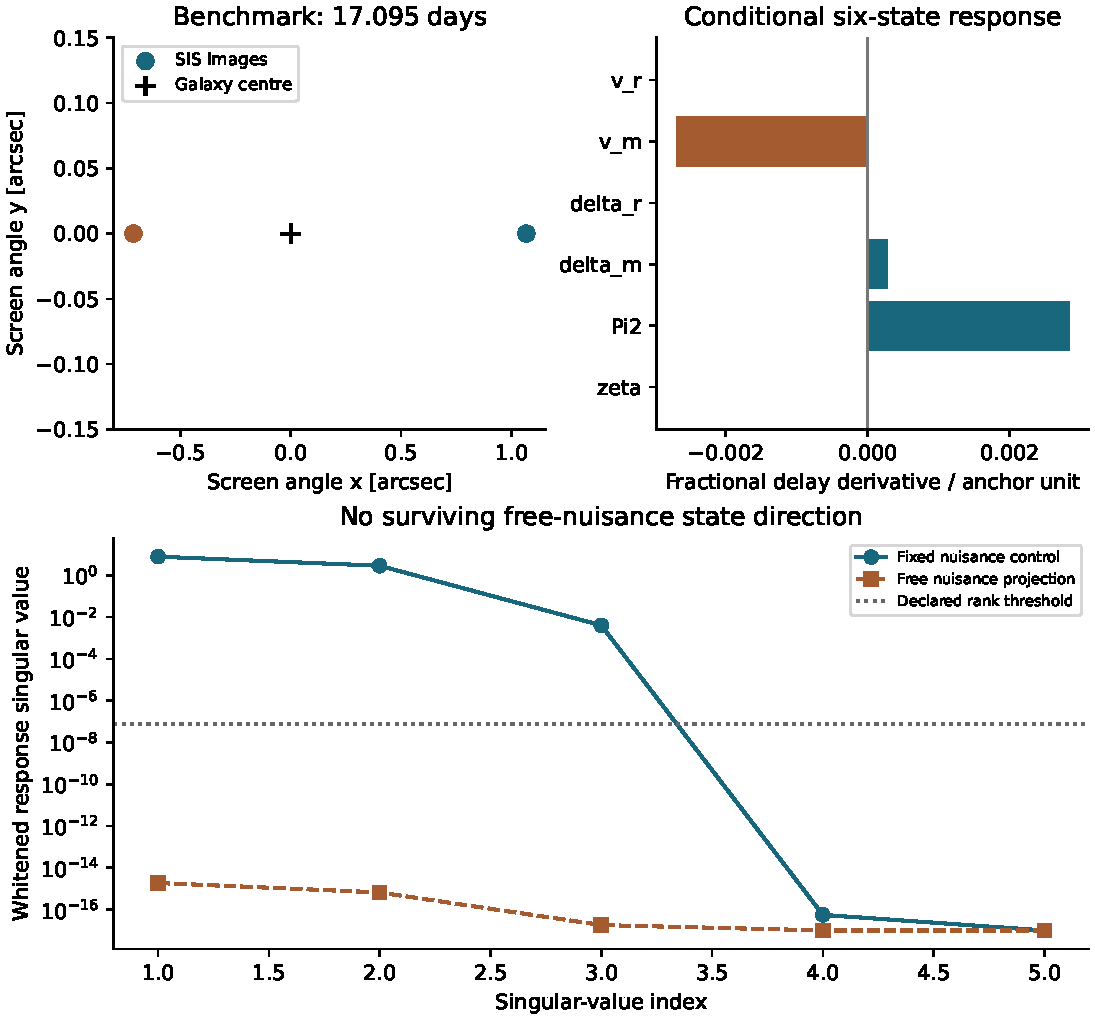
\includegraphics[width=\linewidth]{figures/strong_lensing_comparison.pdf}
 \caption{Executed illustrative comparison and conditional sensitivities.
 The input manifest defines the perturbation, covariance and source
 conventions. These are benchmark calculations rather than an
 observational fit or an action-normalized local envelope prediction.}
 \label{fig:sl-comparison}
 \end{figure}
}{}

The first comparison is valid in geometric optics, linear response of the
smooth geometry, small angles, and the thin, nonrelativistic conventional
galaxy encounter. It excludes caustic crossings under the small finite
variations used in the derivative check. An extended envelope would require
integrating its derived metric through the entrance/exit surfaces before
justifying any thin-plane reduction. This calculation does not supply that
reduction by assumption.

\section{Dependencies and next calculation}
\label{sec:sl-limitations}
The current result separates four kinds of input. The frozen background,
coupled action evolution, conventional encounter solution, compatible
Jacobi/arrival equations and static phase-channel null are derived or
directly evaluated within their stated domain. The incident pulse, selected
spatial profile/axis, source coordinate, galaxy parameters and illustrative
covariance are specified physical or measurement inputs. Unit responses
to physical anchor amplitudes and any independently declared optical
forcing remain conditional sensitivities. The local envelope's
common-domain projected Hessian, nonzero spatial-current reference state,
topographic boundary/source profile, normalized seam export and any
stochastic source covariance remain unresolved.

The next local envelope calculation must evaluate
Eq.~\eqref{eq:sl-static-current} on a specified current state and profile,
project the constrained Hessian in Eq.~\eqref{eq:sl-local-hessian}, and
solve Eq.~\eqref{eq:sl-envelope-chain} with the corresponding boundary
conditions. It can then provide $\delta\hat\psi|_x$ or an extended metric
encounter for Eq.~\eqref{eq:sl-complete-variation}. Smooth cosmological
propagation already included in $D_{ab}$ must remain excluded from that
local encounter. This is the specific dependency needed for testing
an additional interface response or a galaxy-replacement interpretation.

The benchmark and conditional transfer therefore support a controlled
state-dependence experiment: a $17.094532$-day conventional benchmark,
six computed state-response columns, a restricted static phase null and
an explicit failure of identification under the admitted nuisance freedoms.
The rank-zero result is the distinguishability conclusion for this
illustrative configuration. An independently normalized envelope response
requires the local action/state/source closure above and independent
information that removes the relevant degeneracy directions.

The reproducible entry point is
\texttt{python scripts/run\_strong\_lensing\_comparison.py} from the
repository root. The machine-readable result, input hashes and response
arrays are saved under
\texttt{artifacts/strong\_lensing\_first\_comparison\_20261020/}.
The focused tests cover the action projections, six-coordinate transport,
redshift/reciprocity conventions, analytic lens control, complete arrival
derivatives, mass-sheet transformation and correct treatment of unconstrained
directions; 51 focused tests pass. The original broader manuscript remains
a separate source.
